\documentclass{article}
\usepackage[top=1cm, left=1.5cm, right=1.5cm, bottom=1.5cm]{geometry}
\usepackage{graphicx, amsmath, tikz-cd, apacite, amssymb, tcolorbox, wrapfig}
\graphicspath{{./img/}}
\bibliographystyle{apacite}
\setlength{\parindent}{0pt}
\setlength{\parskip}{1em} 
 
\title{Matriz de una Transformación Lineal}
\author{Pablo Dario}
\date{04/01/2024}
 
\begin{document}
\maketitle

Cada transformación lineal de $\mathbb{R}^n$ a $\mathbb{R}^m$ es una transformación matricial \textbf{x} $\longmapsto A$\textbf{x}; la clave para encontrar a $A$ es observar que $T$ esta determinada por su acción sobre las columnas de la matriz identidad de $n \times n, I_n$

\begin{large}
    \textbf{Ejemplo}
\end{large}

Las columnas de $I_2 = \begin{bmatrix} 1 & 0 \\ 0 & 1 \end{bmatrix}$ son $\mathbf{e_1} = \begin{bmatrix} 1 \\ 0 \end{bmatrix}$ y $\mathbf{e_2} = \begin{bmatrix} 0 \\ 1 \end{bmatrix}$ Suponga que $T$ es una transformación lineal de $\mathbb{R}^2$ a $\mathbb{R}^3$ tal que $$T(\mathbf{e_1}) = \left[\begin{array}{r} 5 \\ -7 \\ 2 \end{array}\right] \quad \text{y} \quad T(\mathbf{e_2}) = \left[\begin{array}{r} -3 \\ 8 \\ 0 \end{array}\right]$$

Encuentre la imagen de una \textbf{x} arbitraria en $\mathbb{R}^2$

Así bien creamos un vector \textbf{x} genérico y lo múltplicamos por la matriz identidad, dejándonos: 

\begin{equation*}
    A\mathbf{x} = \begin{bmatrix} 1 & 0 \\ 0 & 1 \end{bmatrix} \begin{bmatrix} x_1 \\ x_2 \end{bmatrix} 
    = x_1 \begin{bmatrix}
        1 \\0 
    \end{bmatrix} + x_2 \begin{bmatrix}
        0 \\ 1
    \end{bmatrix}
    = x_1\mathbf{e_1} + x_2\mathbf{e_2}
\end{equation*}

Como $T$ es una transformación lineal y ya conocemos a los vectores transformados de $\mathbf{e_1}$ y $\mathbf{e_2}$, entonces:

\begin{equation*}
    \begin{aligned}
        T(\mathbf{x}) &= x_1T(\mathbf{e_1}) + x_2T(\mathbf{e_2}) \\
        &= x_1 \left[\begin{array}{r}
        5 \\ -7 \\ 2
        \end{array}\right]
        + x_2 \left[\begin{array}{r}
            -3 \\ 8 \\ 0
        \end{array}\right] 
        = \left[\begin{array}{r}
            5x_1 - 3x_2 \\ -7x_1 + 8x_2 \\ 2x_1 + 0
        \end{array}\right]
    \end{aligned}
\end{equation*}

Por lo tanto, la transformación lineal es: $T(\mathbf{x}) = T( 5x_1 - 3x_2, -7x_1 + 8x_2, 2x_1 + 0)$ y su \textbf{matriz estándar} $A$ es: $$\left[\begin{array}{rr} 5 &-3 \\ -7 & 8 \\ 2 & 0 \end{array}\right]$$

Los pasos anteriores explican porque el conocimiento de $T(\mathbf{e_1})$ y $T(\mathbf{e_2})$ es suficiente para determinar $T(\mathbf{x})$ para cualquier \textbf{x}.

\begin{tcolorbox}[colback=red!10!white, colframe=red!70!black, title=Matriz Estándar]
    Sea $T: \mathbb{R}^n \rightarrow \mathbb{R}^m$ una transformación lineal, existe una única matriz $A$ tal que $$T(\mathbf{x}) = A\mathbf{x} \text{ para toda } \textbf{x} \text{ en } \mathbb{R}^n$$
    
    $A$ es la matriz de $m \times n$ cuya $j-$ésima columna es el vector $T(\mathbf{e_j})$, donde $\mathbf{e_j}$ es la $j-$ésima columna de la matriz identidad en $\mathbb{R}^n$ $$A = \begin{bmatrix}
        T(\mathbf{e_1}) &\dotsb &T(\mathbf{e_n})
    \end{bmatrix}$$
\end{tcolorbox}

El término transformación lineal se enfoca sobre una propiedad de un mapeo, mientras que la transformación matricial describe cómo se implementa tal mapeo.

\begin{large}
    \textbf{Ejemplo 2}
\end{large}

Encuentre la matriz estándar $A$ para la transformación de dilatación $T(\mathbf{x}) = 3\mathbf{x}$, para \textbf{x} en $\mathbb{R}^2$. $$T(\mathbf{e_1}) = 3\mathbf{e_1} = \begin{bmatrix} 3 \\ 0 \end{bmatrix} \quad \text{y} \quad T(\mathbf{e_2}) = 3\mathbf{e_2} = \begin{bmatrix} 0 \\ 3 \end{bmatrix}$$

\begin{equation*}
    \begin{bmatrix}
        3 & 0 \\
        0 & 3
    \end{bmatrix}
\end{equation*}

\begin{large}
    \textbf{Existencia y Unicidad}
\end{large}

\begin{tcolorbox}[colback=blue!10!white,colframe=blue!60!black,title=Existencia]
    Se dice que un mapeo $T: \mathbb{R}^n \rightarrow \mathbb{R}^m$ es \textbf{sobre} $\mathbb{R}^m$ si cada \textbf{b} en $\mathbb{R}^m$ es la imagen de al menos una \textbf{x} en $\mathbb{R}^n$. 

    $T$ mapea $\mathbb{R}^n$ sobre $\mathbb{R}^m$ si y solo si las columnas de $A$ generan a $\mathbb{R}^m$.
\end{tcolorbox}

De manera equivalente, $T$ es sobre $\mathbb{R}^m$ cuando todo el rango de $T$ es codominio $\mathbb{R}^m$. Es decir $T$ mapea $\mathbb{R}^n$ sobre $\mathbb{R}^m$, si para cada \textbf{b} en el codominio $\mathbb{R}^m$, existe al menos una solución de $T(x)=\mathbf{b}$.

El mapeo $T$ no es sobre $\mathbb{R}^m$ cuando existe alguna \textbf{b} en $\mathbb{R}^m$ para la cual la ecuación $T(\mathbf{x}) = \mathbf{b}$ no tiene solución.

\begin{figure}[ht]
  \centerline{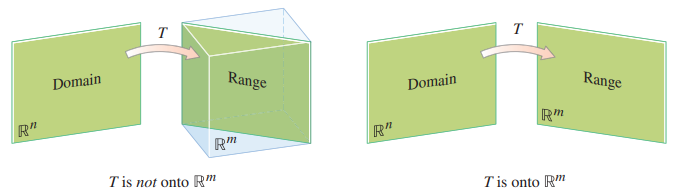
\includegraphics[width=0.8\textwidth]{image22.png}}
  \caption{¿El rango de $T$ es todo $\mathbb{R}^m$?}
\end{figure}

\begin{tcolorbox}[colback=blue!10!white,colframe=blue!60!black,title=Unicidad]
    Se dice que un mapeo $T: \mathbb{R}^n \rightarrow \mathbb{R}^m$  es \textbf{uno a uno} si cada \textbf{b} en $\mathbb{R}^m$ es la imagen de a lo sumo una \textbf{x} en $\mathbb{R}^n$
\end{tcolorbox}

De manera equivalente, $T$ es uno a uno si, para cada \textbf{b} en $\mathbb{R}^m$, la ecuación $T(\mathbf{x}) = \mathbf{b}$ tiene una única solución o ninguna solución.

El mapeo de $T$ no es uno a uno cuando algún \textbf{b} en $\mathbb{R}^m$ es la imagen de más de un vector en $\mathbb{R}^n$. Si no existe tal \textbf{b}, entonces $T$ es uno a uno.

\begin{figure}[ht]
  \centerline{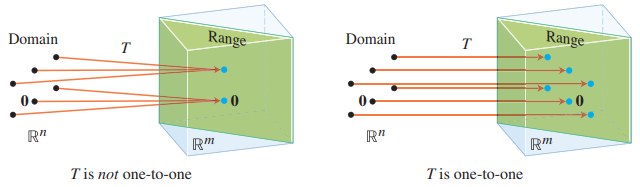
\includegraphics[width=0.8\textwidth]{image23.png}}
  \caption{¿Cada \textbf{b} es la imagen de a lo sumo un vector?}
\end{figure}

\pagebreak

\begin{large}
    \textbf{Ejemplos de Mapeo uno a uno}
\end{large}

\begin{figure}[ht]
  \centerline{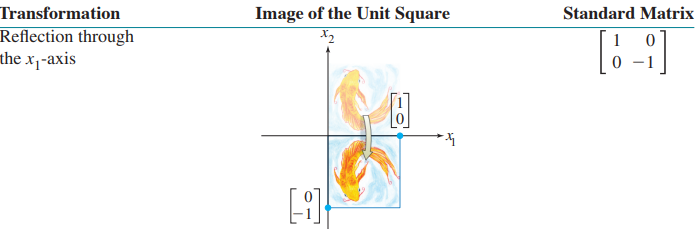
\includegraphics[width=0.8\textwidth]{image24.png}}
  \caption{Reflexiones}
\end{figure}

\begin{figure}[ht]
    \centerline{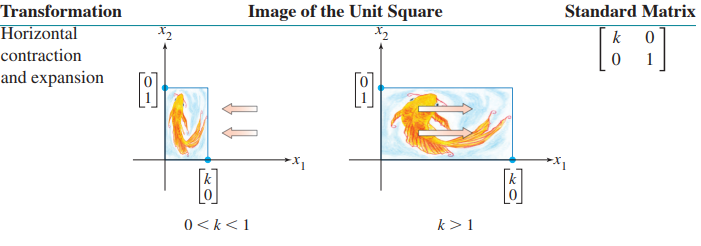
\includegraphics[width=0.8\textwidth]{image25.png}}
    \caption{Contracción y Expansión}
\end{figure}

\begin{figure}[ht]
    \centerline{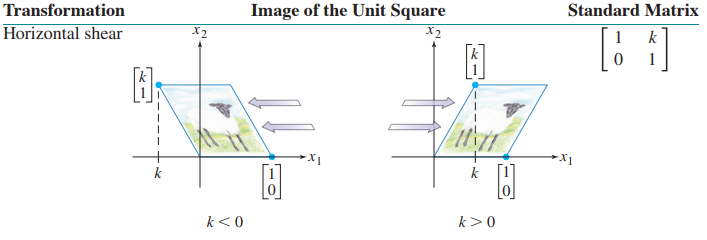
\includegraphics[width=0.8\textwidth]{image26.png}}
    \caption{Trasquilado}
  \end{figure}

\begin{large}
    \textbf{Ejemplo}
\end{large}

Sea $T$ la transformación lineal cuya matriz estándar $A$ es: $$\left[\begin{array}{rrrr}
        1 & -4 & 8 & 1 \\
        0 & 2 & -1 & 3 \\
        0 & 0 & 0 & 5 \\
\end{array}\right]$$ encuentre si $T$ es sobre $\mathbb{R}^4$ y si el mapeo es uno a uno.

Como $A$ está en forma escalonada, podemos ver a la vez que $A$ tiene una posición pivote en cada fila. Para cada \textbf{b} en $\mathbb{R}^3$, la 
ecuación $A\mathbf{x} = \mathbf{b}$ es consistente. En otras palabras, la transformación lineal $T$ mapea $\mathbb{R}^4$ (su dominio) sobre $\mathbb{R}^3$. Sin embargo, ya que la ecuación $A\mathbf{x} = \mathbf{b}$ tiene una variable libre, cada \textbf{b} es la imagen de más de una \textbf{x}. \textbf{Es decir, T no es uno a uno.}

\begin{tcolorbox}[colback=blue!10!white,colframe=blue!60!black,title=Unicidad]
    Sea $T: \mathbb{R}^n \rightarrow \mathbb{R}^m$ una transformación lineal. Entonces $T$ es uno a uno si y solo si la ecuación $T(\mathbf{x}) = 0$ tiene únicamente la solución trivial. 

    $T$ es uno a uno si y solo si las columnas de $A$ son linealmente independientes.
\end{tcolorbox}

\begin{large}
    \textbf{Ejemplo}
\end{large}

Sea $T(x_1, x_2) = (3x_1 + x_2, 5x_1 + 7x_2, x_1 + 3x_2)$ Demuestre que $T$ es una transformación lineal uno a uno. ¿$T$ mapea a $\mathbb{R}^2$ sobre $\mathbb{R}^3$?

\begin{equation*}
    T(\mathbf{x}) = \left[\begin{array}{rr}
        3x_1 + x_2\\
        5x_1 + 7x_2\\
        x_1  + 3x_2
    \end{array}\right]
    = \begin{bmatrix}
        3 & 1\\
        5 & 7\\
        1 & 3
    \end{bmatrix} \begin{bmatrix}
        x_1 \\ x_2
    \end{bmatrix}
\end{equation*}

Las columnas de $A$ son linealmente independientes porque no son múltiplos entre sí; por lo tanto $T$ es uno a uno. Por otro lado las columnas de $A$ generan a $\mathbb{R}^3$ si y solo si $A$ tiene 3 posiciones pivote; podemos observar rápidamente que esto es imposible ya que $A$ solo tiene 2 columnas. Así las columnas de $A$ no generan a $R^3$ y la transformación linealmente asociada no es sobre $\mathbb{R}^3$.

\begin{tcolorbox}[colback=red!10!white, colframe=red!70!black, title=Resumen]
    \begin{itemize}
        \item[-]Un mapeo $T: \mathbb{R}^n \rightarrow \mathbb{R}^m$ es \textbf{sobre} $\mathbb{R}^m$ si cada \textbf{b} en $\mathbb{R}^m$ es la imagen de al menos una \textbf{x} en $\mathbb{R}^n$. Es decir $T$ mapea $\mathbb{R}^n$ sobre $\mathbb{R}^m$, si para cada \textbf{b} en el codominio $\mathbb{R}^m$, existe al menos una solución de $T(x)=\mathbf{b}$.
        \item[-] $T$ mapea $\mathbb{R}^n$ sobre $\mathbb{R}^m$ si y solo si las columnas de $A$ generan a $\mathbb{R}^m$.
        \item[-] Un mapeo $T: \mathbb{R}^n \rightarrow \mathbb{R}^m$  es \textbf{uno a uno} si cada \textbf{b} en $\mathbb{R}^m$ es la imagen de a lo sumo una \textbf{x} en $\mathbb{R}^n$, o si, para cada \textbf{b} en $\mathbb{R}^m$, la ecuación $T(\mathbf{x}) = \mathbf{b}$ tiene una única solución o ninguna solución
        \item[-] $T$ es uno a uno si y solo si la ecuación $T(\mathbf{x}) = 0$ tiene únicamente la solución trivial, por lo que si hay una variable libre la transformación $T$ no es uno a uno, o bien si hay más columnas que filas en la matriz $A$. 
        \item[-] $T$ es uno a uno si y solo si las columnas de $A$ son linealmente independientes.        
    \end{itemize}
\end{tcolorbox}

\end{document}